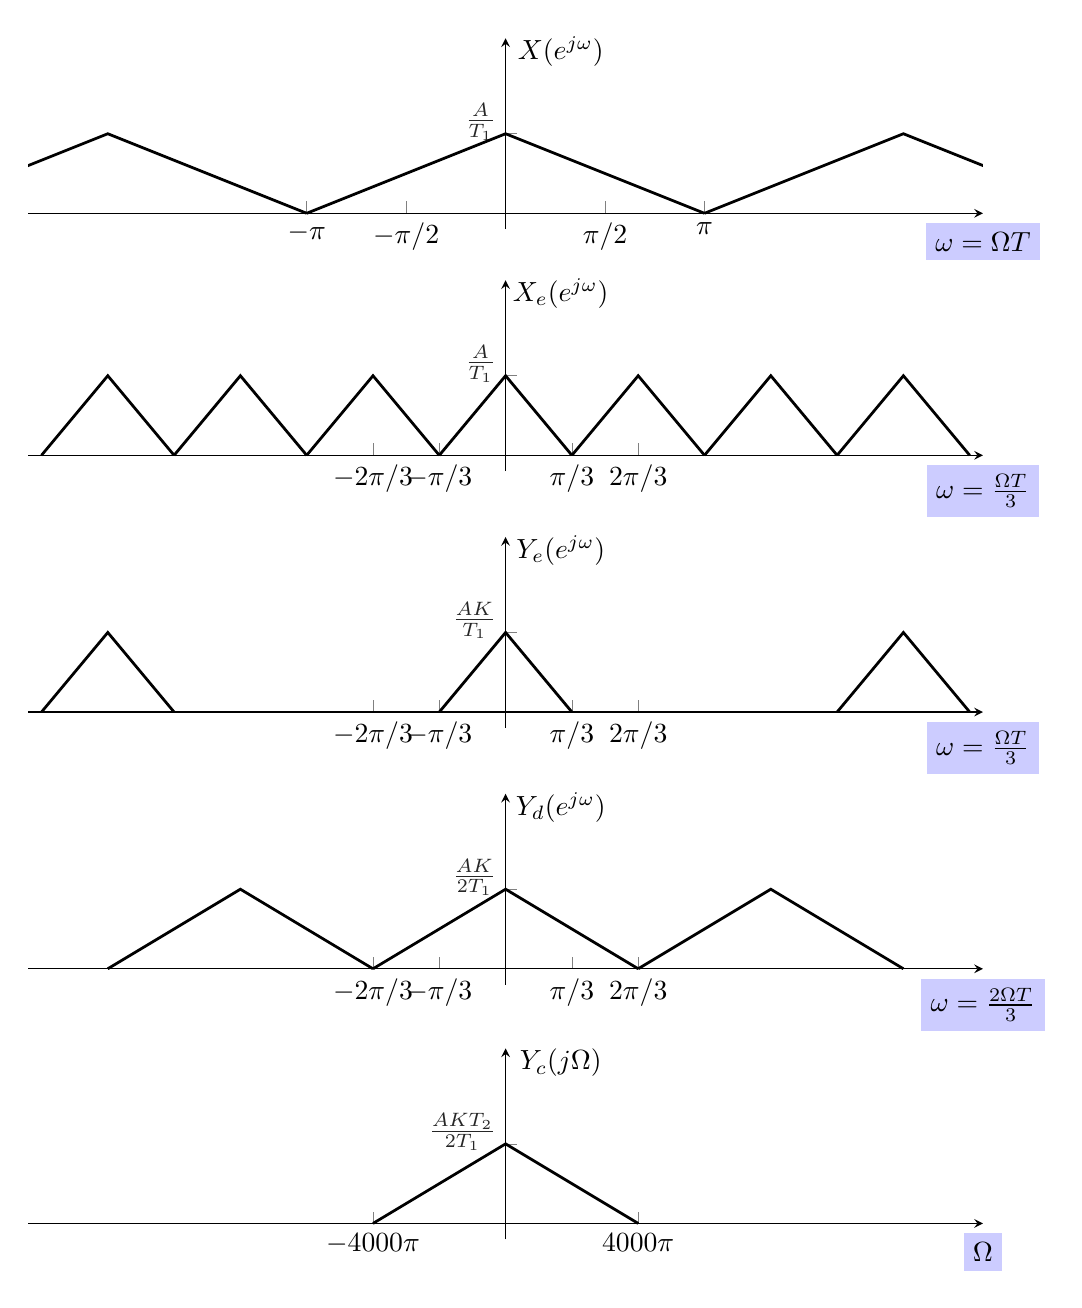
\begin{tikzpicture}
\begin{axis}[
name=plot1,
%at=(plot2.below south east), anchor=above north east,
axis lines*=middle,
enlargelimits = true,
clip=true,
scale only axis,
width=\textwidth,
height=0.2\textwidth,
ymin=0, ymax=2,
xmin=-16, xmax=16,
axis line style={->,>=stealth},
xlabel={\tikz[baseline]{\node[fill=blue!20,anchor=base] (t1) {$\omega=\Omega T$};}},
ylabel={$X(e^{j\omega})$},
every axis x label/.style={
	at={(ticklabel* cs:1)},
	%xshift=0.2cm,
	anchor=north,
},
every axis y label/.style={
	at={(ticklabel* cs:0.8)},
	anchor=south,
	xshift=0.7cm,
},
ytick={1},
yticklabels={$\frac{A}{T_1}$},
yticklabel style={yshift=0.15cm},
xtick={-8, -4, 4, 8},
xticklabels={$-\pi$, $-\pi/2$, $\pi/2$, $\pi$}, 
every outer y axis line/.append style={white!15!black},
every y tick label/.append style={font=\color{white!15!black}},
legend style={draw=white!15!black,fill=white,legend cell align=left}]
\def\fs{16}
\foreach \k in {-1, 0, 1}{
	\addplot[solid, line width=1pt] coordinates {(-8+\k*\fs, 0) (0+\k*\fs, 1) (8+\k*\fs, 0)};	
}
\end{axis}

\begin{axis}[
name=plot2,
at=(plot1.below south east), anchor=above north east,
axis lines*=middle,
enlargelimits = true,
clip=true,
scale only axis,
width=\textwidth,
height=0.2\textwidth,
ymin=0, ymax=2,
xmin=-16, xmax=16,
axis line style={->,>=stealth},
xlabel={\tikz[baseline]{\node[fill=blue!20,anchor=base] (t1) {$\omega = \frac{\Omega T}{3}$};}},
ylabel={$X_e(e^{j\omega})$},
every axis x label/.style={
	at={(ticklabel* cs:1)},
	%xshift=0.2cm,
	anchor=north,
},
every axis y label/.style={
	at={(ticklabel* cs:0.8)},
	anchor=south,
	xshift=0.7cm,
},
ytick={1},
yticklabels={$\frac{A}{T_1}$},
yticklabel style={yshift=0.15cm},
xtick={-5.3333, -2.6667, 2.6667, 5.3333},
xticklabels={$-2\pi/3$, $-\pi/3$, $\pi/3$, $2\pi/3$},
every outer y axis line/.append style={white!15!black},
every y tick label/.append style={font=\color{white!15!black}},
legend style={draw=white!15!black,fill=white,legend cell align=left}]
\def\fs{5.3333}
\foreach \k in {-3, -2, -1, 0, 1, 2, 3}{
	\addplot[solid, line width=1pt] coordinates {(-8/3+\k*\fs, 0) (0+\k*\fs, 1) (8/3+\k*\fs, 0)};	
}
\end{axis}

\begin{axis}[
name=plot3,
at=(plot2.below south east), anchor=above north east,
axis lines*=middle,
enlargelimits = true,
clip=true,
scale only axis,
width=\textwidth,
height=0.2\textwidth,
ymin=0, ymax=2,
xmin=-16, xmax=16,
axis line style={->,>=stealth},
xlabel={\tikz[baseline]{\node[fill=blue!20,anchor=base] (t1) {$\omega = \frac{\Omega T}{3}$};}},
ylabel={$Y_e(e^{j\omega})$},
every axis x label/.style={
	at={(ticklabel* cs:1)},
	%xshift=0.2cm,
	anchor=north,
},
every axis y label/.style={
	at={(ticklabel* cs:0.8)},
	anchor=south,
	xshift=0.7cm,
},
ytick={1},
yticklabels={$\frac{AK}{T_1}$},
yticklabel style={yshift=0.15cm},
xtick={-5.3333, -2.6667, 2.6667, 5.3333},
xticklabels={$-2\pi/3$, $-\pi/3$, $\pi/3$, $2\pi/3$},
every outer y axis line/.append style={white!15!black},
every y tick label/.append style={font=\color{white!15!black}},
legend style={draw=white!15!black,fill=white,legend cell align=left}]
\def\fs{5.3333}
\foreach \k in {-3, 0,  3}{
	\addplot[solid, line width=1pt] coordinates {(-8/3+\k*\fs, 0) (0+\k*\fs, 1) (8/3+\k*\fs, 0)};	
}
\end{axis}

\begin{axis}[
name=plot4,
at=(plot3.below south east), anchor=above north east,
axis lines*=middle,
enlargelimits = true,
clip=true,
scale only axis,
width=\textwidth,
height=0.2\textwidth,
ymin=0, ymax=2,
xmin=-16, xmax=16,
axis line style={->,>=stealth},
xlabel={\tikz[baseline]{\node[fill=blue!20,anchor=base] (t1) {$\omega = \frac{2\Omega T}{3}$};}},
ylabel={$Y_d(e^{j\omega})$},
every axis x label/.style={
	at={(ticklabel* cs:1)},
	%xshift=0.2cm,
	anchor=north,
},
every axis y label/.style={
	at={(ticklabel* cs:0.8)},
	anchor=south,
	xshift=0.7cm,
},
ytick={1},
yticklabels={$\frac{AK}{2T_1}$},
yticklabel style={yshift=0.15cm},
xtick={-5.3333, -2.6667, 2.6667, 5.3333},
xticklabels={$-2\pi/3$, $-\pi/3$, $\pi/3$, $2\pi/3$},
every outer y axis line/.append style={white!15!black},
every y tick label/.append style={font=\color{white!15!black}},
legend style={draw=white!15!black,fill=white,legend cell align=left}]
\def\fs{10.6667}
\foreach \k in {-1, 0, 1}{
	\addplot[solid, line width=1pt] coordinates {(-16/3+\k*\fs, 0) (0+\k*\fs, 1) (16/3+\k*\fs, 0)};	
}
\end{axis}


\begin{axis}[
name=plot5,
at=(plot4.below south east), anchor=above north east,
axis lines*=middle,
enlargelimits = true,
clip=true,
scale only axis,
width=\textwidth,
height=0.2\textwidth,
ymin=0, ymax=2,
xmin=-16, xmax=16,
axis line style={->,>=stealth},
xlabel={\tikz[baseline]{\node[fill=blue!20,anchor=base] (t1) {$\Omega$};}},
ylabel={$Y_c(j\Omega)$},
every axis x label/.style={
	at={(ticklabel* cs:1)},
	%xshift=0.2cm,
	anchor=north,
},
every axis y label/.style={
	at={(ticklabel* cs:0.8)},
	anchor=south,
	xshift=0.7cm,
},
ytick={1},
yticklabels={$\frac{AKT_2}{2T_1}$},
yticklabel style={yshift=0.15cm},
xtick={-5.3333, 5.3333},
xticklabels={$-4000\pi$, $4000\pi$},
every outer y axis line/.append style={white!15!black},
every y tick label/.append style={font=\color{white!15!black}},
legend style={draw=white!15!black,fill=white,legend cell align=left}]
\def\fs{10.6667}
\foreach \k in {0}{
	\addplot[solid, line width=1pt] coordinates {(-16/3+\k*\fs, 0) (0+\k*\fs, 1) (16/3+\k*\fs, 0)};	
}
\end{axis}
\end{tikzpicture}
